\documentclass[biblatex,aspectratio=169,11pt]{mybeamer}

\usetikzlibrary{backgrounds,calc,decorations.pathreplacing,fit,matrix,patterns,positioning,shapes,shapes.multipart,tikzmark}
\makeatletter
\let\@@magyar@captionfix\relax
\makeatother

%Add page footer
\setbeamertemplate{footline}[text line]{%
  \parbox{\linewidth}{\vspace*{-8pt}\hfill CS6290 Privacy-enhancing Technologies\hfill\insertpagenumber}}
\setbeamertemplate{navigation symbols}{}

\title{A Preliminary Investigation into Storageless Blockchain}
\author{Yang Ji}
\date{April 15, 2019}

\addbibresource{ref.bib}

\begin{document}

\maketitle%
\PrintTOC%

\section{Introduction}

\begin{frame}{Background}
  \begin{itemize}
    \item In cryptocurrency, peer-to-peer payment transactions are asynchronously broadcasted and recorded in an ordered ledger.
    \item Consensus protocol requires nodes to validate new transactions. 
    \item e.g. To send 6 ETC from Alice to Bob requires that Alice has at least 6 ETC.
    \item Simply querying the history on the blockchain is infeasible and insecure due to the large size of blocks.
    \item For that reason, most cryptocurrency nodes need to locally maintain the \alert{validation state}, which means downloading all past transactions/accounts.
  \end{itemize}
\end{frame}

\begin{frame}{Background}
  \begin{itemize}
    \item In Bitcoin, Zcash and Komodo, \alert{validation state} is a set of immutable coins called \alert{UTXO} (unspent transaction output)
  \end{itemize}
  \vspace{-1em}
  \begin{figure}
    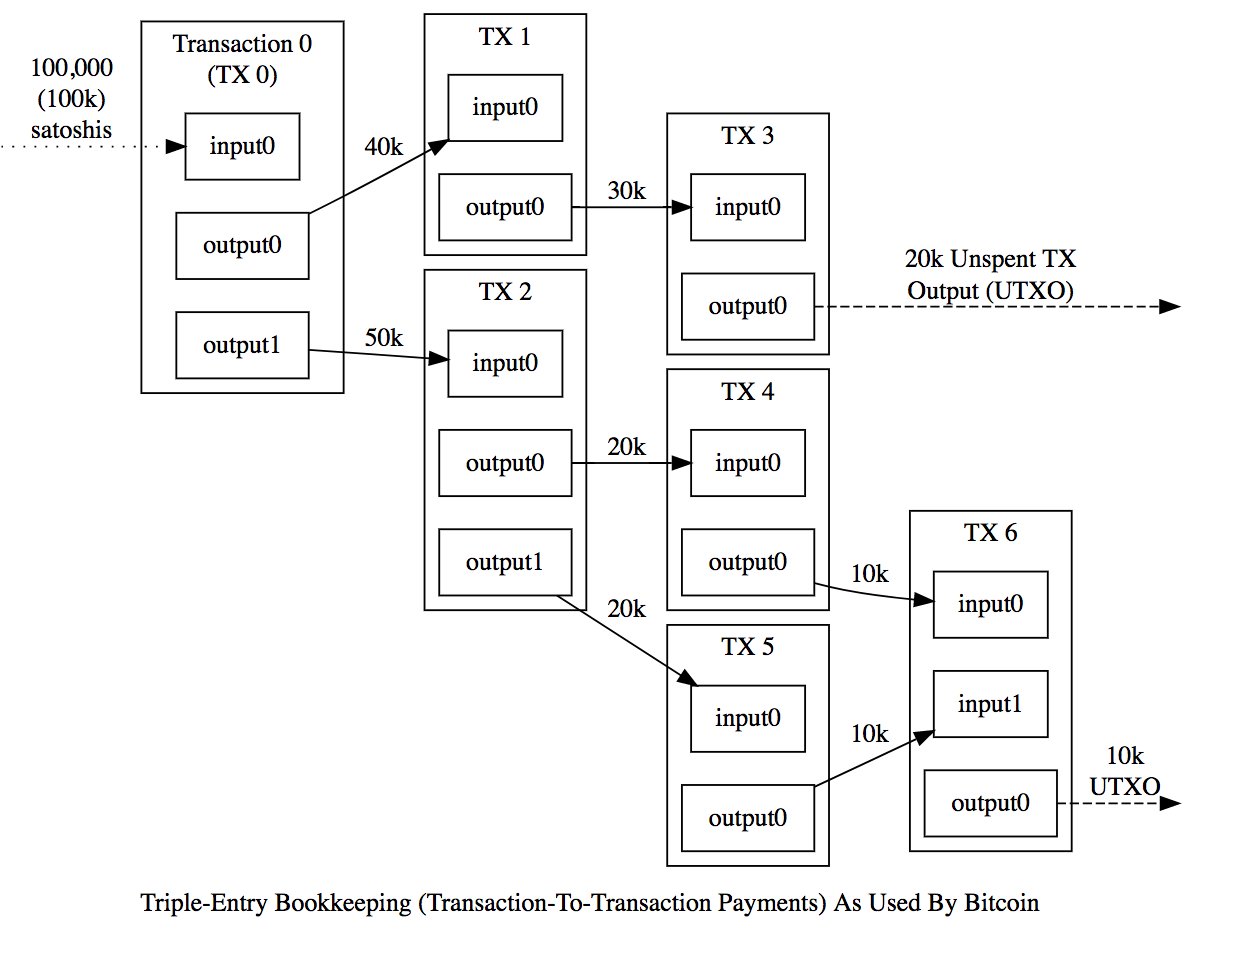
\includegraphics[width=0.45\linewidth]{figs/utxo.png}
    \caption{UTXO Model}
  \end{figure}
\end{frame}


\begin{frame}{Background}
  \begin{itemize}
    \item In Ethereum, Nxt and Bitshares organize \alert{validation state} as a set of mutable (and potential long-living) \alert{accounts}.
  \end{itemize}
  \vspace{-1em}
  \begin{figure}
    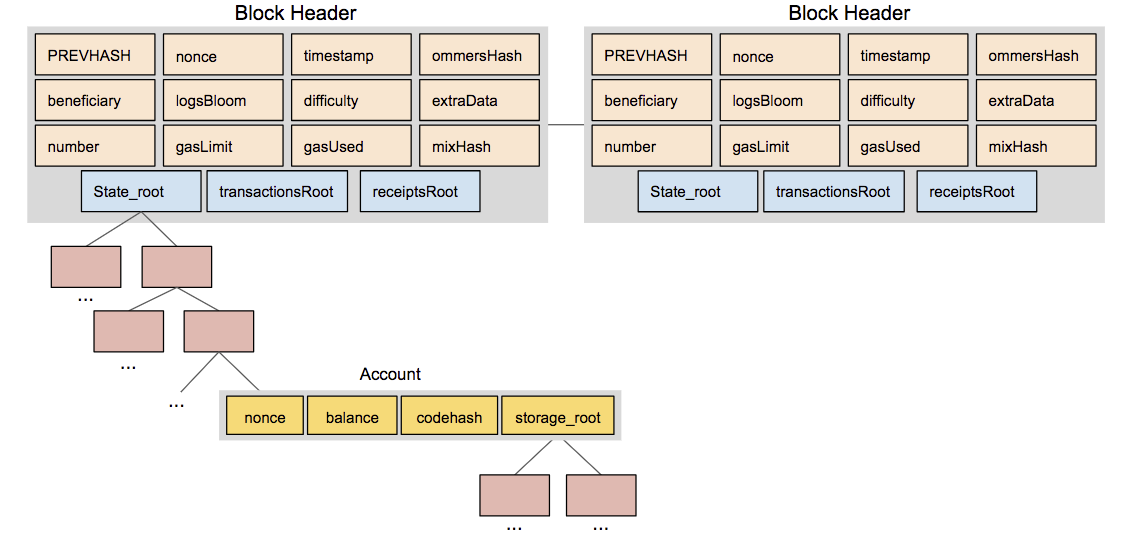
\includegraphics[width=0.7\linewidth]{figs/account.png}
    \caption{Account-based Model}
  \end{figure}
\end{frame}

\begin{frame}{Background}
  \begin{itemize}
    \item Other cryptocurrencies
  \end{itemize}
  \vspace{-1em}
  \begin{figure}
    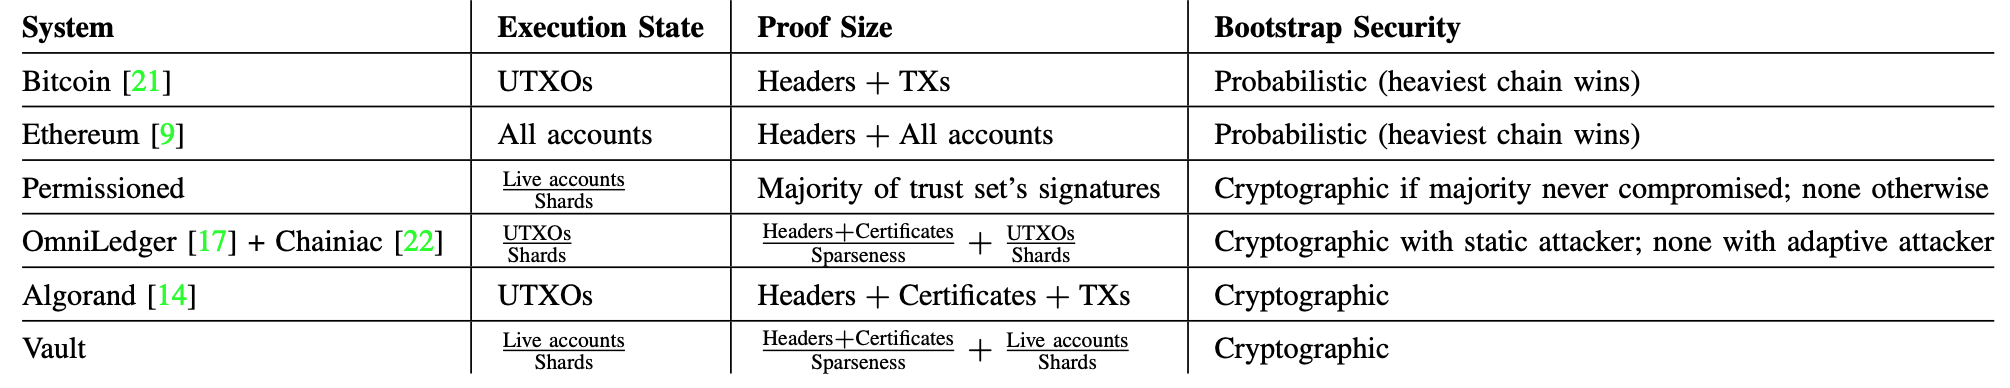
\includegraphics[width=0.9\linewidth]{figs/summary.png}
    \caption{Comparison of different cryptocurrency models }
  \end{figure}
\end{frame}

\begin{frame}{Motivation}
  \begin{itemize}
    \item Maintaining ledger state is cumbersome from the perspectives of \alert{storage} and \alert{bootstrapping}
    \begin{itemize}
       \item Large size (Bitcoin is around 150 GB and Ethereum has exceeded 400 GB)
       \item Data storage size is linear with block number and could grow substantially in the coming years
       \item Slow disk I/O operations (LevelDB or RocksDB)
       \item DoS attack (adversarially-crafted transactions that need massive of disk accesses)
       \item Increase the possibility of centralization in blockchains.
    \end{itemize}
    \item Several people including Peter Todd and Mike Hearn also talked about \alert{storageless clients} for Bitcoin in 2013.
    \item It thus appears that we need to compress the \alert{ledger history}.
  \end{itemize}
\end{frame}

\begin{frame}{Difficulty}
  \begin{itemize}
    \item State set growth is driven by a number of factors, including the following fact.
     \begin{itemize}
       \item For \alert{Bitcoin}, there are massive of merge inputs, lost coins and dust outputs.
       \item For \alert{Ethereum}, smart contract inadvertently created many \alert{zero-balance accounts}~(account for around 38\%).
     \end{itemize}
    \item Based on these, a na\"ive way is to prune and clean `useless' dust coins/accounts.
    \item However, there is little incentive to carry it out for many reasons:
     \begin{itemize}
       \item Dust coins can't be economically spent and have other use cases.
       \item We can't delete zero accounts because nodes need to keep track of the sequence number ("nonce")~\cite{wood2014ethereum}.
     \end{itemize}
    \item Redesigning index structures and storage mode has limited improvement.
  \end{itemize}
\end{frame}


\section{Analysis of Existing Works}

\begin{frame}{Possible Solutions}
  \begin{itemize}[<+->]
    \item Method 1: \alert{Storage Rent}
     \begin{itemize}[<+->]
       \item Miners could know and update ledger state by outsourcing local database to third party or sharing common files with other miners in IPFS system.
       \item \textbf{Drawbacks:} The operation cost is very high; less competitive; low I/O operations.
     \end{itemize}
     \item Method 2: \alert{Sharding}
      \begin{itemize}[<+->]
        \item Partition the whole blockchain/storage into many shardings like Zilliqa~\cite{zilliqa2017zilliqa} and Omniledger~\cite{kokoris2018omniledger}.
        \item \textbf{Drawbacks:} Security issues; Incentive mechanism;
      \end{itemize}
     \item Method 3: \alert{Merging Transactions} 
      \begin{itemize}[<+->]
        \item Record fewer transactions using payment channels e.g. lightning network~\cite{poon2016bitcoin}
        \item \textbf{Drawbacks:} Only support pairwise payment relationship;
      \end{itemize}
     \item Method 4: \alert{Compacting Blocks}~\cite{poelstra2016mimblewimble}
  \end{itemize}
\end{frame}


\section{Stateless Blockchain}

\begin{frame}{Stateless Blockchain}
  \begin{itemize}
   \item This design concept of \alert{Stateless Blockchain} is referred to Peter Todd's blog post~\cite{Tod}. 
   \item Nodes might participate in transaction validation without storing the entire state of the ledger.
   \item Transaction would include membership proofs for all its input.
   \item A node would only need to store the current state and verify transactions by checking membership proofs against accumulator state.
   \item Many optimized schemes are put forward in the forum, such as TXO commitment~\cite{MMR} and asynchronous accumulator~\cite{reyzin2016efficient} for dual accumulator.
 \end{itemize}
\end{frame}

\begin{frame}{Architecture}
  \begin{figure}
    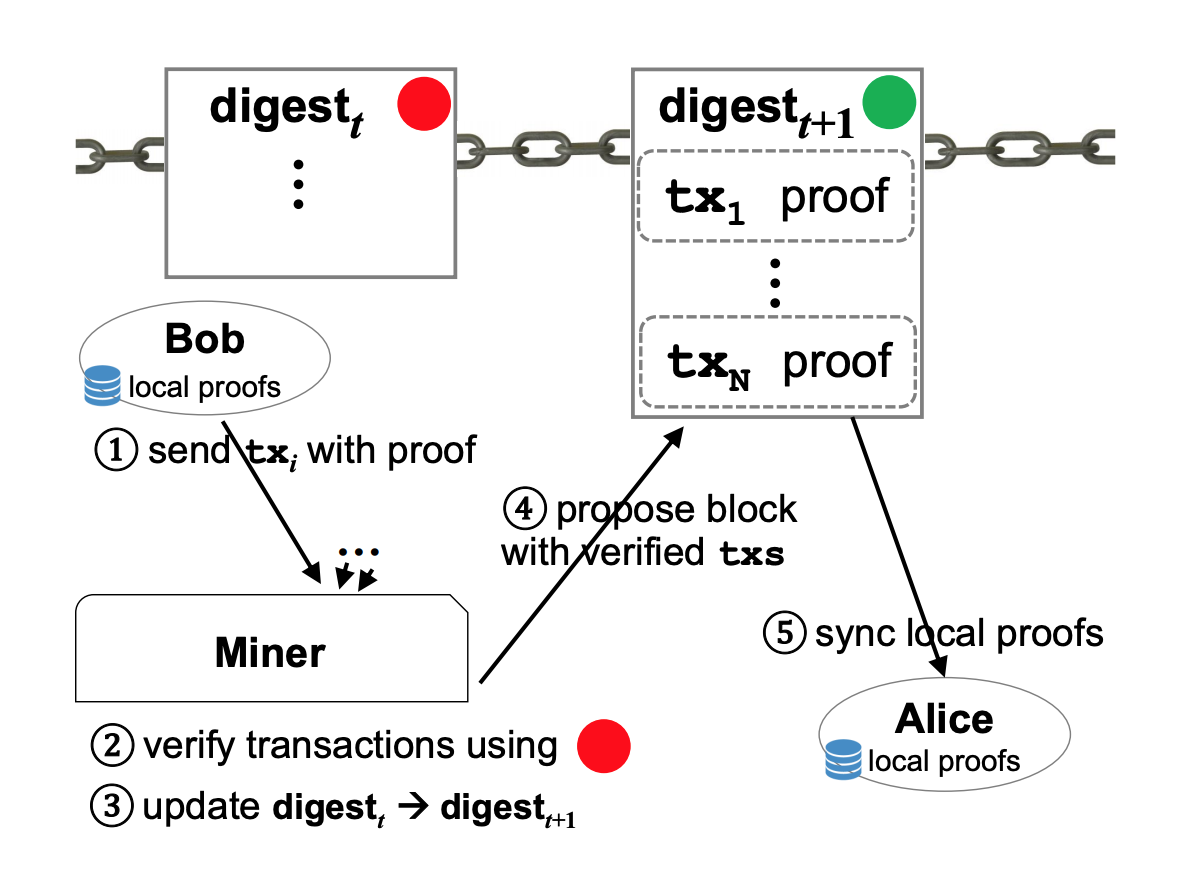
\includegraphics[width=0.6\linewidth]{figs/Edrax-arch.png}
    \caption{System Architecture}
  \end{figure}
\end{frame}

\metroset{subsectionpage=simple}
\subsection{\fullcite{leung2019vault}}

\begin{frame}{Vault Techniques}
  \begin{itemize}
    \item \textbf{Vault:} Reducing the cost of storage and bootstrapping without weakening security guarantees.
  \end{itemize}
  \vspace{-2em}
  \begin{table}[]
    \begin{tabular}{|l|l|l|}
    \hline
    Approach                                                                                 & Challenge                                                               & Vault’s Solution                                                        \\ \hline
    \begin{tabular}[c]{@{}l@{}}Reduce state\\ transmitted:\\ Garbage collection\end{tabular} & \begin{tabular}[c]{@{}l@{}}Transaction replay\\ attacks\end{tabular}    & \begin{tabular}[c]{@{}l@{}}Force transactions\\ to expire\end{tabular}  \\ \hline
    \begin{tabular}[c]{@{}l@{}}Reduce state\\ transmitted:\\ Shard state\end{tabular}        & \begin{tabular}[c]{@{}l@{}}Small shards lose\\ security\end{tabular}    & \begin{tabular}[c]{@{}l@{}}Adaptive Merkle\\ Tree sharding\end{tabular} \\ \hline
    \begin{tabular}[c]{@{}l@{}}Reduce size of\\ state proof:\\ Compress history\end{tabular} & \begin{tabular}[c]{@{}l@{}}Attacker tampers\\ with history\end{tabular} & \begin{tabular}[c]{@{}l@{}}Succinct\\ certificates\end{tabular}         \\ \hline
    \end{tabular}
  \end{table}
\end{frame}

\begin{frame}{Vault: Forcing Transactions to Expire}
  \vspace{-3em}
  \begin{itemize}
    \item All transactions contain the fields \alert{$t_{issuance}$} and \alert{$t_{expiry}$}.
    \item We define $0 \leq t_{expiry} - t_{issuance} \leq t_{max}$
    \item The choice of $T_{max}$ affects two considerations.
     \begin{itemize}
       \item The block number of transactions to detect double spend.
       \item Expiration mechanism requires the issuer to reissue expired transactions.
     \end{itemize}
    \item Support off-chain payment channels e.g. Lightning Network.
  \end{itemize}
\end{frame}

\begin{frame}{Vault: Sharding Balance Storage}
  \vspace{-2em}
  \begin{figure}
    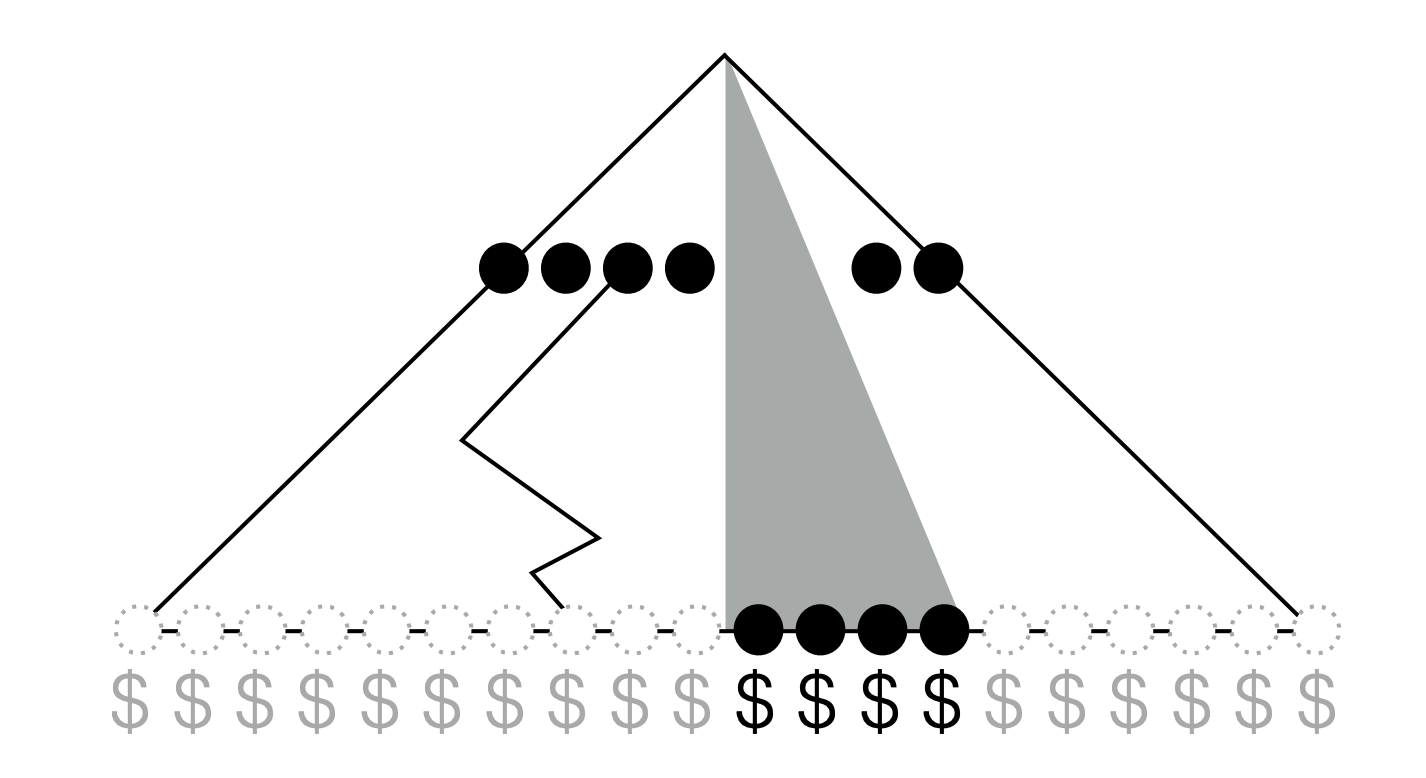
\includegraphics[width=0.5\linewidth]{figs/vault-sharding.png}
  \end{figure}
  \vspace{-2em}
  \begin{itemize}
    \item \textbf{Shard Witness:} Transactions include Merkle witness for source and destination accounts.
    \item \textbf{Updating Witness:} The witness could be updated without requiring the issuer to resign the entire transaction.
    \item \textbf{Adaptive Sharding: } Truncating witness.
  \end{itemize}
\end{frame}

\begin{frame}{Vault: Compressing History}
  \begin{itemize}
    \item Skipping Blocks
    \begin{figure}
      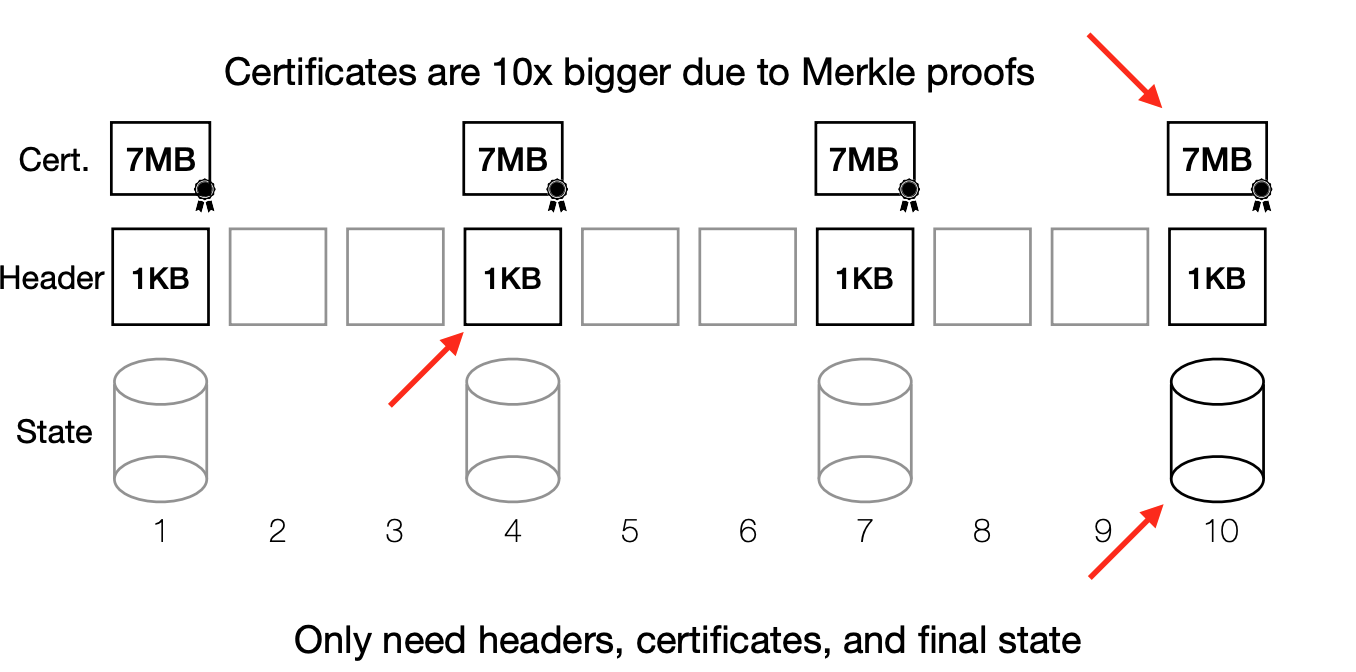
\includegraphics[width=0.5\linewidth]{figs/skip-block.png}
      \caption{An illustration for skipping blocks}
    \end{figure}
    \item Shrinking Certificates
  \end{itemize}
\end{frame}

\subsection{\fullcite{chepurnoy2018edrax}}



\begin{frame}{General Idea}
  \begin{itemize}
    \item Represent UTXO as a sparse Merkle tree.
    \item For account-based model, we can use MHT to represent the mapping of $pk \leftrightarrow balance$
    \item Store the MHT root in the block as digest
    \item However, during \texttt{SPEND}, we need the Merkle proofs of both sender and receiver
    \item Instead, we can use \alert{vector commitment} to represent account-balance mapping.
  \end{itemize}
\end{frame}

\begin{frame}{Edrax in account-based model}
  \vspace{-2em}
  \begin{itemize}
    \item Edrax requires an \alert{one-time setup phase}. 
      \item Each block stores a validation digest
        \begin{itemize}
          \item A vector commitment digest whose mapping is $i \leftrightarrow h(\textsf{PK}) || balance$
          \item A counter $cnt_t$ which indicates the number of existing accounts
        \end{itemize}
      \item Clients store vector commitment proof $\pi$ w.r.t.\ their index $i$
      \item The index $i$ is assigned when client submits an \alert{\texttt{INIT} transaction} $[\texttt{INIT}, pk]$
        \begin{itemize}
          \item Miner verifies transaction signature
          \item Client is assigned to $i \gets cnt_t$
          \item Miner updates $cnt_{t+1} \gets cnt_t + 1$ and a new digest \\
            $\textsf{UpdateDigest}(dig, cnt, h(\textsf{PK}) || 0, upk_{cnt})$
          \item Clients synchronize proofs accordingly using UpdateProof
        \end{itemize}
  \end{itemize}
\end{frame}

\begin{frame}{\texttt{SPEND} Transaction}
  \begin{itemize}
    \item To spend $\delta$ to client with public key $\textsf{PK}_b = pk_b || j || upk_j$
    \item Client sends transaction $[\textsf{PK}_a, \textsf{PK}_b, v, \pi_i, v']$ with signature $sig$
    \item Miner verifies:
      \begin{itemize}
        \item $sig$ is valid
        \item $v \leq v'$
        \item $\textsf{Verify}(dig_t, i, h(\textsf{PK}_a) || v', \pi_i, vrk)$ passes
      \end{itemize}
    \item Miner updates digest
      \begin{itemize}
        \item $dig' \gets \textsf{UpdateDigest}(dig_t, i, -v, upk_i)$
        \item $dig_{t+1} \gets \textsf{UpdateDigest}(dig', j, v, upk_j)$
      \end{itemize}
    \item Clients synchronize proofs accordingly using UpdateProof
  \end{itemize}
\end{frame}

\begin{frame}{Discussion}
  \begin{itemize}[<+->]
    \item Either authenticated data structure or vector commitment provides a \alert{short binding commitment} to a set of elements together with short \alert{membership/non-membership proof}.
    \item In essence, stateless blockchain reduces the storage burden for performing transaction validation by \alert{sacrificing communication overhead and assigning miners' tasks to clients}.
    \item Possible optimizations: 
     \begin{itemize}[<+->]
       \item Shorten membership proof size
       \item aggregate membership proofs for a batch of transactions~\cite{boneh2018batching}
     \end{itemize}
  \end{itemize}
\end{frame}

\begin{frame}{Possible Works and Directions}
  \begin{itemize}[<+->]
    \item More efficient authenticated data structure instead of sparse merkle tree
    \item Local proof synchronization by miner
    \item Introducing proof-serving nodes
    \item Supporting smart contracts in the stateless setting
    \item Adding privacy to account-based model
  \end{itemize}
\end{frame}

\nocite{*}
\PrintRef%
\PrintQA%

\end{document}
